\documentclass[border=1pt]{standalone}
\usepackage{tikz}
\usepackage{luatexja}

\begin{document}
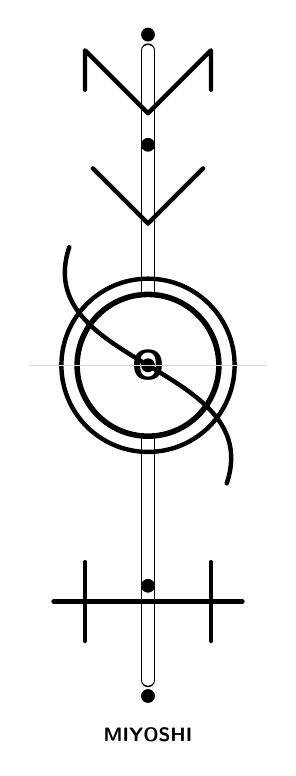
\begin{tikzpicture}[line width=1.6pt, line cap=round, line join=round]
    % メイン軸 (I)
    \draw[double, double distance=4pt, line width=0.5pt] (0, -4.0) -- (0, 4.0);
    
    % M (最上部)
    \draw (-0.8, 3.5) -- (-0.8, 4.0) -- (0, 3.2) -- (0.8, 4.0) -- (0.8, 3.5);
    
    % Y (中央上部)
    \draw (-0.7, 2.5) -- (0, 1.8) -- (0.7, 2.5);
    
    % O (中央コア)
    \draw[line width=2pt, fill=white] (0, 0) circle (0.9);
    \node[font=\sffamily\bfseries, scale=1.5] at (0,0) {O};
    \draw (0,0) circle (1.1);
    
    % S (中央を貫くうねり)
    \draw (-1.0, 1.5) .. controls (-1.5, 0) and (1.5, 0) .. (1.0, -1.5);

    % H (下部)
    \draw (-0.8, -2.5) -- (-0.8, -3.5);
    \draw (0.8, -2.5) -- (0.8, -3.5);
    \draw (-1.2, -3.0) -- (1.2, -3.0);
    
    % 装飾ドットと細線
    \foreach \y in {4.2, 2.8, 0, -2.8, -4.2} \fill (0, \y) circle (2.5pt);
    \draw[gray!30, line width=0.4pt] (-1.5, 0) -- (1.5, 0);

    % 縦書きテキスト
    \node[anchor=north, font=\sffamily\bfseries, scale=0.7] at (0, -4.5) {M\\I\\Y\\O\\S\\H\\I};
\end{tikzpicture}
\end{document}
